\section{Experimental Results}
\label{sec:experimental_results}

In this section, we describe the datasets, validation protocols and experimental results. 

\begin{table*}[!htbp]
\centering
\caption{Composition of the Datasets}
\label{tab:dataset_composition}
\resizebox{\linewidth}{!}{%
    \begin{tabular}{l|ccc|ccc|ccc}
    \multirow{2}{*}{{\bf Dataset}} & \multicolumn{3}{c|}{\bf Train} & \multicolumn{3}{c|}{\bf Test known} & \multicolumn{3}{c}{\bf Test unknown} \\
     & {\bf Live} & {\bf Contacts} & {\bf Printouts} & {\bf Live} & {\bf Contacts} & {\bf Printouts} & {\bf Live} & {\bf Contacts} & {\bf Printouts} \\ \hline\hline
    Clarkson & 2,469 & 1,122 & 1,346 & 1,485 & 765 & 908 & 638 & 494 & 144 \\ \hline
    IIITD-WVU & 2,250 & 1,000 & 3,000 & -- & -- & -- & 702 & 701 & 2,806 \\ \hline
    Notre Dame & 600 & 600 & -- & 900 & 900 & -- & 900 & 900 & -- \\ \hline
    Warsaw & 1,844 & -- & 2,669 & 974 & -- & 2,016 & 2,350 & -- & 2,160 \\ \hline\hline
    Combined & 7,163 & 2,722 & 7,015 & 3,359 & 1,665 & 2,924 & 4,590 & 2,095 & 5,110 \\
    \end{tabular}%
    }
\end{table*}

\subsection{Datasets}
\label{sec:dataset}

Our work was performed on datasets made available in the Iris Liveness Detection Competition 2017 \cite{Yambay2017}. There is one set from each of four universities involved --- Clarkson University, Warsaw University of Technology, IIITD-WVU and University of Notre Dame.

The Clarkson dataset \cite{Yambay2014, Yambay2015, Yambay2017} contains images of live irises, textured contact lenses, and iris printouts. The Warsaw dataset \cite{Yambay2017} comprises images of live irises and iris printouts. 
The Notre Dame dataset \cite{Doyle2015} contains images of live irises without textured contact lenses and of irises wearing textured contact lenses. Finally, the IIITD-WVU dataset \cite{Kohli2013, Gupta2014, Yadav2014, Kohli2016} contains images of live irises, textured contact lenses, iris printouts, and printouts of textured contact lenses.
Table \ref{tab:dataset_composition} summarizes the composition of the datasets. For some of our experiments, we also formed a merged dataset by combining the four sets, which we will refer to as the ``Combined'' dataset. The original cross-validation partitioning was kept the same in the ``Combined'' dataset.

\begin{figure*}[!htb]
    \centering
    \begin{subfigure}[b]{0.99\linewidth}
        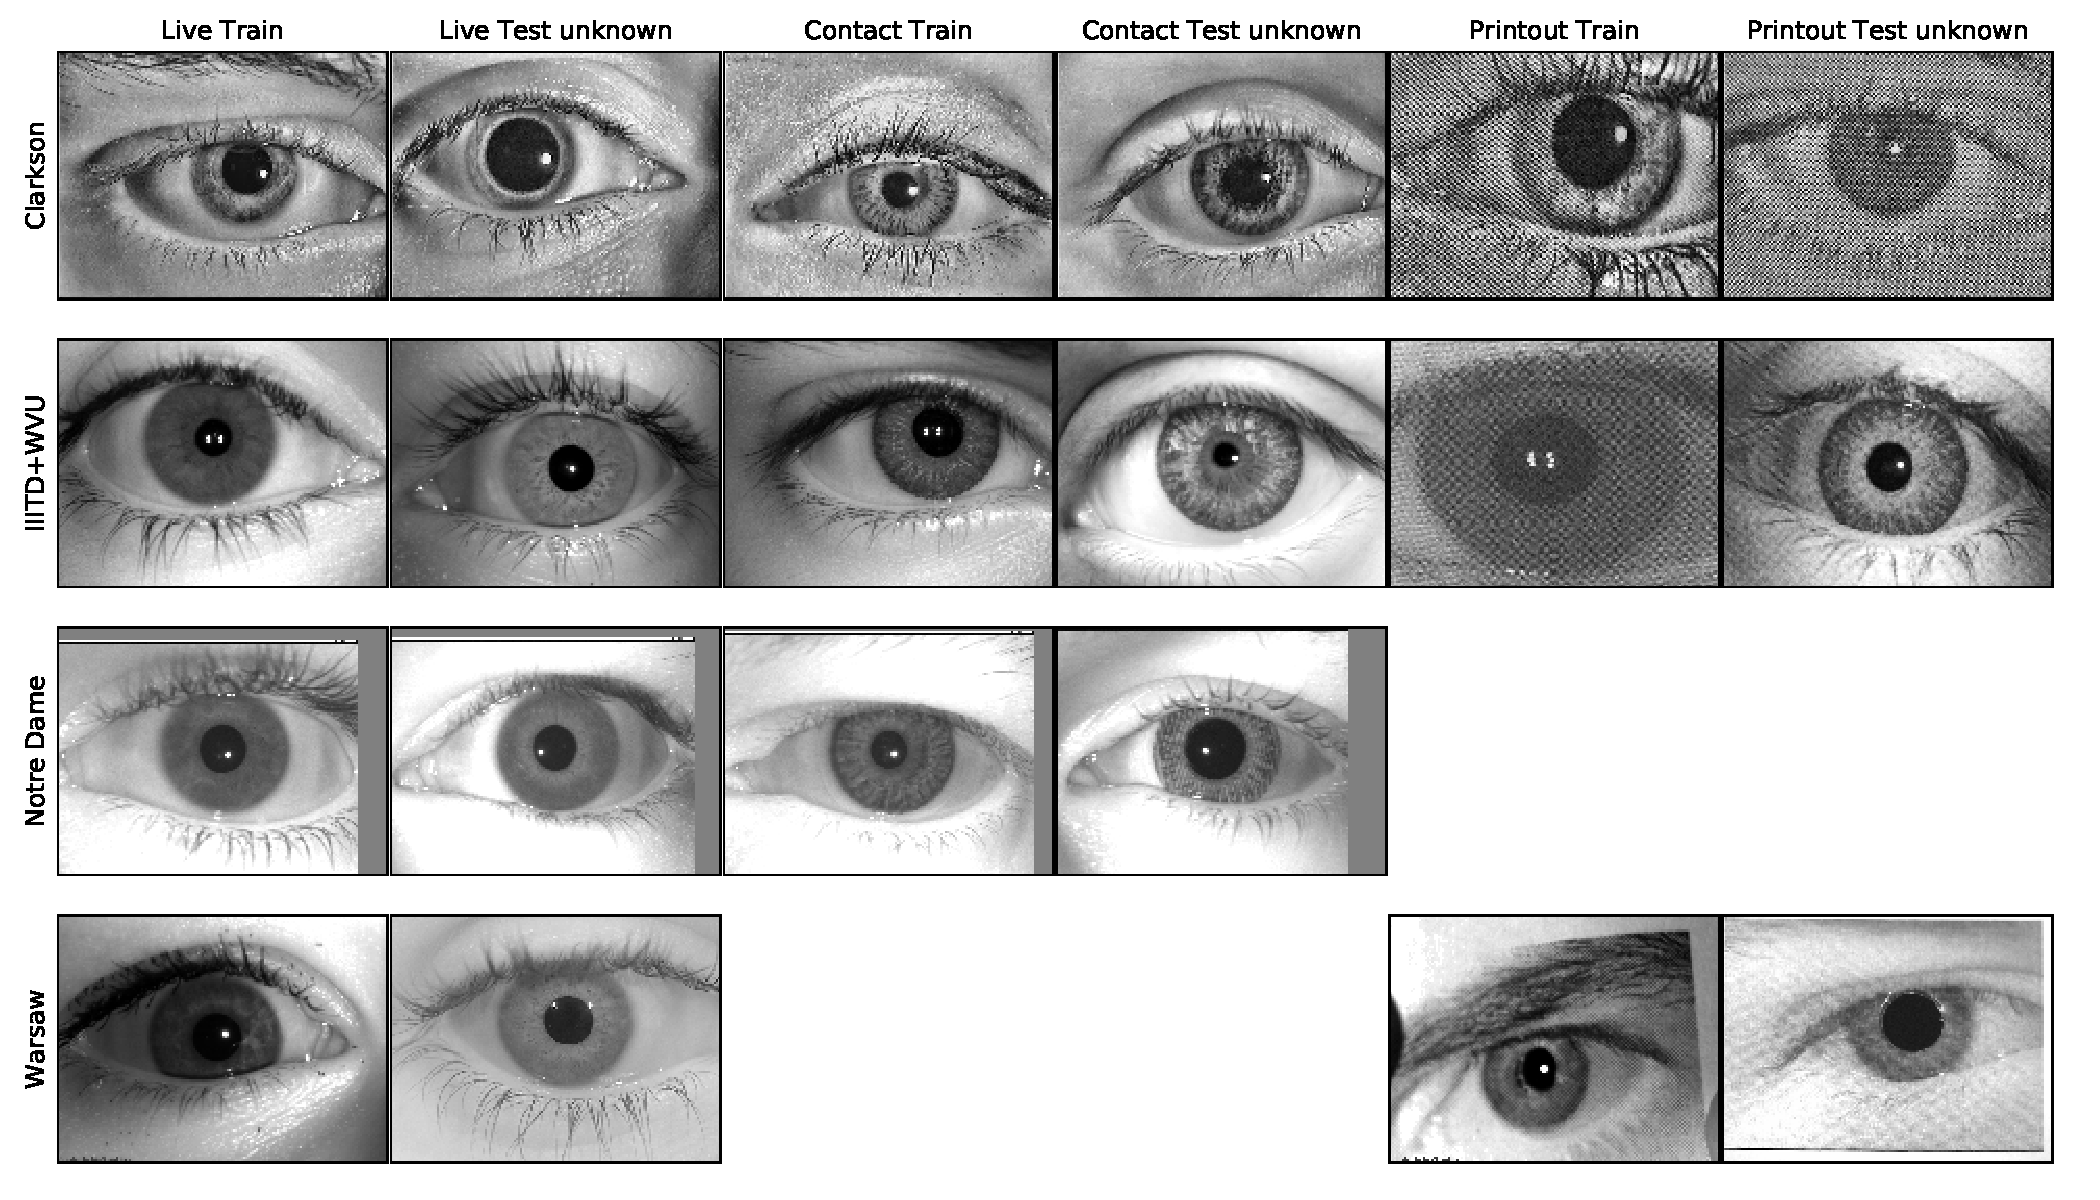
\includegraphics[width=\linewidth, 
                         trim=0.4cm 0.5cm 0.8cm 0.3cm,clip]{imgsamples.pdf}
    \end{subfigure}
    \caption{Image samples from all datasets, from the \emph{train} and \emph{unknown} partitions. The difference between train and unknown images, especially in the case of attacks, illustrates situations where classifiers commonly fail.}
    \label{fig:img_samples}
\end{figure*}

Each dataset is composed of a \emph{train} partition, made available to the participants to facilitate training their algorithms, and a \emph{test} partition, not distributed before the competition was ended, and used by the organizers to evaluate the submissions. LivDet-Iris 2017 co-organizers marked their test samples to form two groups of images. In the first group, referred to as \emph{test known}, both live images and images of artifacts had the same ``known'' properties as train samples. The images belonging to a second group, \emph{test unknown}, have different, or ``unknown'', properties than pictures included in the train subsets. Competition organizers applied different strategies when producing the \emph{test unknown} samples. Clarkson University included visible-light image printouts and new patterns of textured contact lenses, Warsaw University of Technology used different equipment to prepare and photograph iris printouts. The images of patterned contact lenses offered by University of Notre Dame are of different brands than those in the train set. Finally, the whole test partition of the IIITD-WVU benchmark is considered as \emph{test unknown}, since it was collected by a different institution (WVU) than the train set (IIITD), by a different sensor, and included outdoor acquisitions. Figure \ref{fig:img_samples} shows sample images of each dataset.

To keep our evaluation protocol compliant with LivDet-Iris 2017, training of our methods uses solely pre-defined training partitions of the datasets, while the final performance is estimated both on the \emph{test known} and \emph{test unknown} partitions.



% ==========================================================================================================
\subsection{Experimental Protocol}
\label{sec:experimental_protocol}

Our experiments followed the LivDet-Iris 2017 competition protocol \cite{livdet2017}, using the same datasets and train/test partitions as described in Section \ref{sec:dataset}. A sub-partition consisting of a randomly selected 20\% of the images from each train set was created to serve as a validation set during training. The system is trained to perform binary classification: authentic iris images should be labeled as \emph{live}, while attack images (textured contact lenses, printouts of live images or printouts of textured contact lenses) should be labeled as \emph{attack}.

We measure the performance of classifiers using four metrics: 

\begin{itemize}
    \item \emph{Accuracy}, which is the ratio between the number of correctly classified images and the total number of images classified,
    \item \emph{Bona-Fide Presentation Classification Error Rate} (BPCER), which is the proportion of \emph{live} images that were incorrectly classified as \emph{attacks},  
    \item \emph{Attack Presentation Classification Error Rate} (APCER), which is the proportion of \emph{attack} images incorrectly classified as \emph{live} samples, and
    \item \emph{Half Total Error Rate} (HTER), which corresponds to the average of BPCER and APCER.
\end{itemize}

BPCER and APCER error rates were defined by ISO/IEC 30107-3 \cite{ISO_30107-3_2017} and adopted in LivDet-Iris 2017 for evaluation of submissions. The \emph{accuracy} and HTER are used in the training stage for ranking the obtained solutions.

The CNN classifiers output a liveness score in the range of $\langle 0,1 \rangle$ and the decision threshold was 0.5, as defined in the LivDet-Iris 2017 protocol. The source-code to reproduce all of our experiments is available to researchers \footnote{Available on GitHub: \url{https://github.com/akuehlka/mvlc_ipad}.}.


% ==========================================================================================================
\subsection{Evaluation of BSIF Representations and CNN-based Detectors}
\label{sec:evaluation_bsif_cnns}

% The first part of our work was to train and evaluate 61 lightweight CNNs, which act as primary predictors in our system. 
% The number of CNNs used correspond to the 60 BSIF representations of the input image and one raw image representation, upon which each network will be trained.

\begin{figure}[!hb]
    \centering
    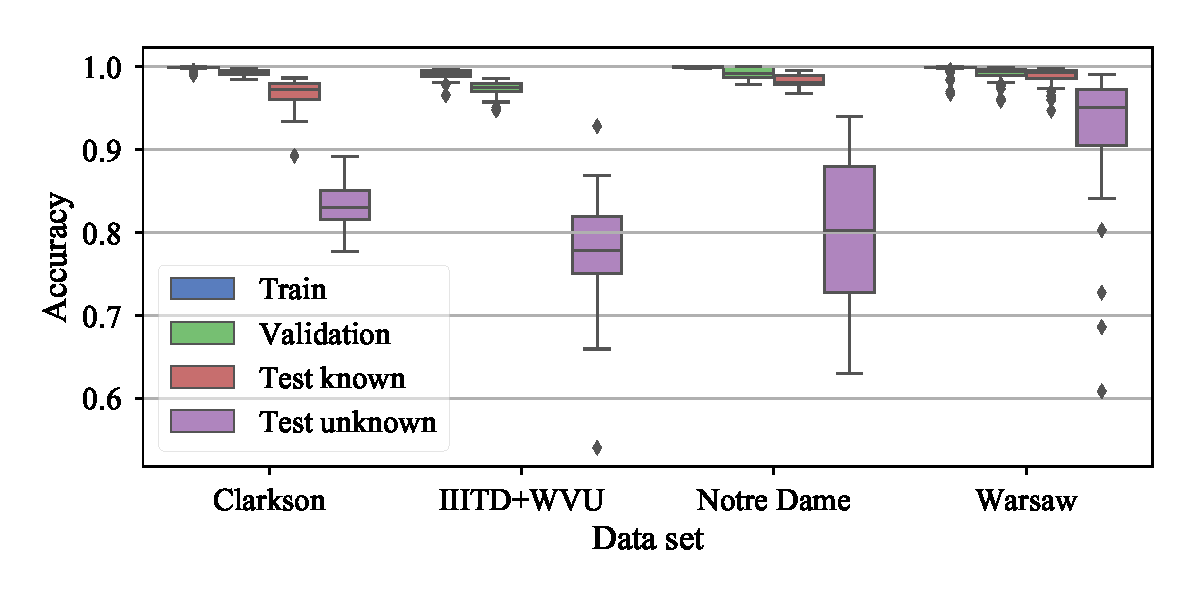
\includegraphics[
        width=\linewidth,
        trim=0.6cm 0.7cm 0.5cm 0.5cm
        ]{Individual_predictor_acc}
    \caption{Distribution of classification accuracies for individual CNN predictors, on each dataset and partition.}
    \label{fig:individual_accuracy}
\end{figure}

The first part of our work was to train and evaluate 61 lightweight CNNs, which act as primary predictors in our system.
As it could be anticipated, individual CNN predictors result in a very good accuracy on the \emph{train} and \emph{test known} partitions, but they do not generalize well to \emph{test unknown} data. This can be seen in Fig.~\ref{fig:individual_accuracy}, which shows the distribution of accuracies obtained by all 61 CNN-based predictors.

Since the CNN is different for different feature descriptors, one can assume the variation in performance is caused by the ability of such descriptors to capture particular textures of the images. This may suggest that some filters are particularly good at classifying a certain type of attack (a certain textured lens brand or a type of a printout), but they are inadequate for others. The proposed method identifies good predictors and aggregates them in order to create a more robust cross-dataset PAD system.

Table ~\ref{tab:individual_top3} shows the top three CNN classifiers on each data set. The size of the BSIF filters that performed best in each data set may offer some insight about the types of features that are being used for classification. While CNN predictors achieved very high accuracy on Warsaw dataset using BSIF filters of size ranging from 5 to 7, the best performing filters on Notre Dame dataset are of size ranging from 3 to 5, while for Clarkson data the best filters are larger, and their size ranges from 7 to 15. The range of BSIF filter sizes that performed best in IIITD+WVU goes from 5 through 17, which is consistent with the wide diversity of images found in this dataset.

It is important to observe a basic difference in the datasets: while Warsaw attack images are printouts, Notre Dame's attack images are textured contact lenses. On the other hand, Clarkson and IIITD+WVU attack subsets are composed of a mix of textured contacts and printouts. Another fact that should be noted is that these data sets do not have similar proportions regarding the number of samples for each class in each partition. As an example, while there are only 144 printouts ($\sim11\%$) in Clarkson unknown, IIITD+WVU has 2,806 ($\sim66\%$) printouts in the same partition. These differences in data set composition may help to explain how different BSIF filter sizes achieve different ranges of performance for each dataset.

% \begin{figure}[!b]
%     \centering
%     \includegraphics[
%         width=\linewidth,
%         trim=0.1cm 0.3cm 0.1cm 0.2cm
%     ]{Individual_top3}
%     \caption{Classification accuracy of the top 3 predictors for each dataset.}
%     \label{fig:individual_top3}
% \end{figure}

\begin{table}[!b]
\centering
\caption{Classification accuracy (\%) of the top 3 predictors for each dataset on the \textit{Test unknown} partition.}
\label{tab:individual_top3}
\begin{tabular}{cccc}
\hline
Dataset                     & BSIF Filter & Accuracy & HTER    \\ \hline \hline
\multirow{3}{*}{Clarkson}   & 15x15x11    & 87.08\%  & 12.91\% \\
                            & 07x07x10    & 82.69\%  & 17.29\% \\
                            & 13x13x12    & 80.74\%  & 19.25\% \\ \midrule
\multirow{3}{*}{IIITD+WVU}  & 05x05x07    & 81.87\%  & 47.45\% \\
                            & 09x09x11    & 78.69\%  & 27.03\% \\
                            & 17x17x07    & 77.62\%  & 19.41\% \\ \midrule
\multirow{3}{*}{Notre Dame} & 05x05x11    & 71.78\%  & 28.22\% \\
                            & 05x05x10    & 69.11\%  & 30.89\% \\
                            & 03x03x06    & 67.83\%  & 32.17\% \\ \midrule
\multirow{3}{*}{Warsaw}     & 05x05x11    & 98.00\%  & 2.08\% \\ 
                            & 07x07x12    & 93.84\%  & 6.24\% \\
                            & 05x05x08    & 91.95\%  & 8.26\% \\
\hline
\end{tabular}
\end{table}

% ==========================================================================================================
\subsection{Fusion Evaluation}
\label{sec:eval_simple_fusion}

% After obtaining classification results from all 61 CNN predictors, we try to combine them in an ensemble, based on the premise that a collection of classifiers is typically more accurate than a simple classifier. 
Before deciding that a more elaborate method for fusion would be required, we experimented with basic methods. Table \ref{tab:simple_fusion} summarizes results of four basic fusion methods: Random Forest (RF), Majority Voting (MV), Best-to-worst Weighted Voting by Accuracy (BWWVA), and by Importance (BWWVI).
%
While there is no clear trend towards a specific fusion method, all of them seem to perform best in specific datasets and partitions. With regard to the data sets, the same trend seen in the CNN predictors happens here: Warsaw had the highest accuracy, followed by IIITD+WVU, Clarkson, and Notre Dame. However, in some cases simple fusion led to an obvious gain in accuracy that was not always the case: some fusion methods were not able to obtain a better result than the best individual classifier, typically in the unknown test partitions.

\begin{table*}[!htb]
\centering
\caption{Results for four simple fusion strategies on the \emph{test known} (K) and \emph{test unknown} (U) partitions; best HTERs in bold.
% %
% \todo[inline]{The same suggestion I did in the Fig. 5}
% %
}
\label{tab:simple_fusion}
\resizebox{\textwidth}{!}{%
\huge
\begin{tabular}{ll|cccc|cccc|cccc|cccc} \hline
                            &   & \multicolumn{4}{c|}{\textbf{RF}}           & \multicolumn{4}{c|}{\textbf{MV}}           & \multicolumn{4}{c|}{\textbf{BWWVA}}        & \multicolumn{4}{c}{\textbf{BWWVI}}        \\ \cline{3-18}
                            &   & Accuracy & APCER & BPCER & HTER  & Accuracy & APCER & BPCER & HTER  & Accuracy & APCER & BPCER & HTER  & Accuracy & APCER & BPCER & HTER  \\ \hline
\multirow{2}{*}{Clarkson}   & K & 97.74    & 4.45  & 0.74  & 2.59  & 99.48    & 0.00  & 0.87  & \textbf{0.44}  & 99.44    & 0.00  & 0.94  & 0.47  & 99.40    & 0.09  & 0.94  & 0.52  \\
                            & U & 78.70    & 41.94 & 0.63  & 21.28 & 85.59    & 28.17 & 0.63  & 14.40 & 86.37    & 26.60 & 0.63  & \textbf{13.61} & 85.75    & 27.70 & 0.78  & 14.24 \\ \hline
\multirow{2}{*}{IIITD+WVU}  & K & -        & -     & -     & -     & -        & -     & -     & -     & -        & -     & -     & -     & -        & -     & -     & -     \\
                            & U & 83.34    & 15.94 & 20.23 & \textbf{18.08} & 83.82    & 12.83 & 32.91 & 22.87 & 84.25    & 12.29 & 33.05 & 22.67 & 83.06    & 9.21  & 55.56 & 32.38 \\ \hline
\multirow{2}{*}{Notre Dame} & K & 99.44    & 0.44  & 0.67  & \textbf{0.56}  & 99.33    & 0.22  & 1.11  & 0.67  & 99.39    & 0.33  & 0.89  & 0.61  & 99.27    & 0.44  & 1.00  & 0.72  \\
                            & U & 85.11    & 29.33 & 0.44  & \textbf{14.89} & 82.39    & 34.22 & 1.00  & 17.61 & 81.61    & 35.78 & 1.00  & 18.39 & 82.28    & 34.44 & 1.00  & 17.72 \\ \hline
\multirow{2}{*}{Warsaw}     & K & 99.80    & 0.05  & 0.51  & 0.28  & 99.87    & 0.04  & 0.31  & 0.18  & 99.87    & 0.05  & 0.31  & 0.18  & 99.90    & 0.00  & 0.30  & \textbf{0.15}  \\
                            & U & 99.51    & 0.32  & 0.64  & \textbf{0.48}  & 99.49    & 0.37  & 0.64  & 0.50  & 99.51    & 0.37  & 0.59  & \textbf{0.48}  & 99.46    & 0.23  & 0.81  & 0.52  \\ \hline
\end{tabular}
}%
\end{table*}


RF fusion was the most successful method, outperforming the others in three situations. 
With the exception of BWWVA, which tied with RF in the unknown partition of Warsaw, all other fusion methods were best in a single dataset/partition.
%
\begin{figure*}[b]
    \centering
    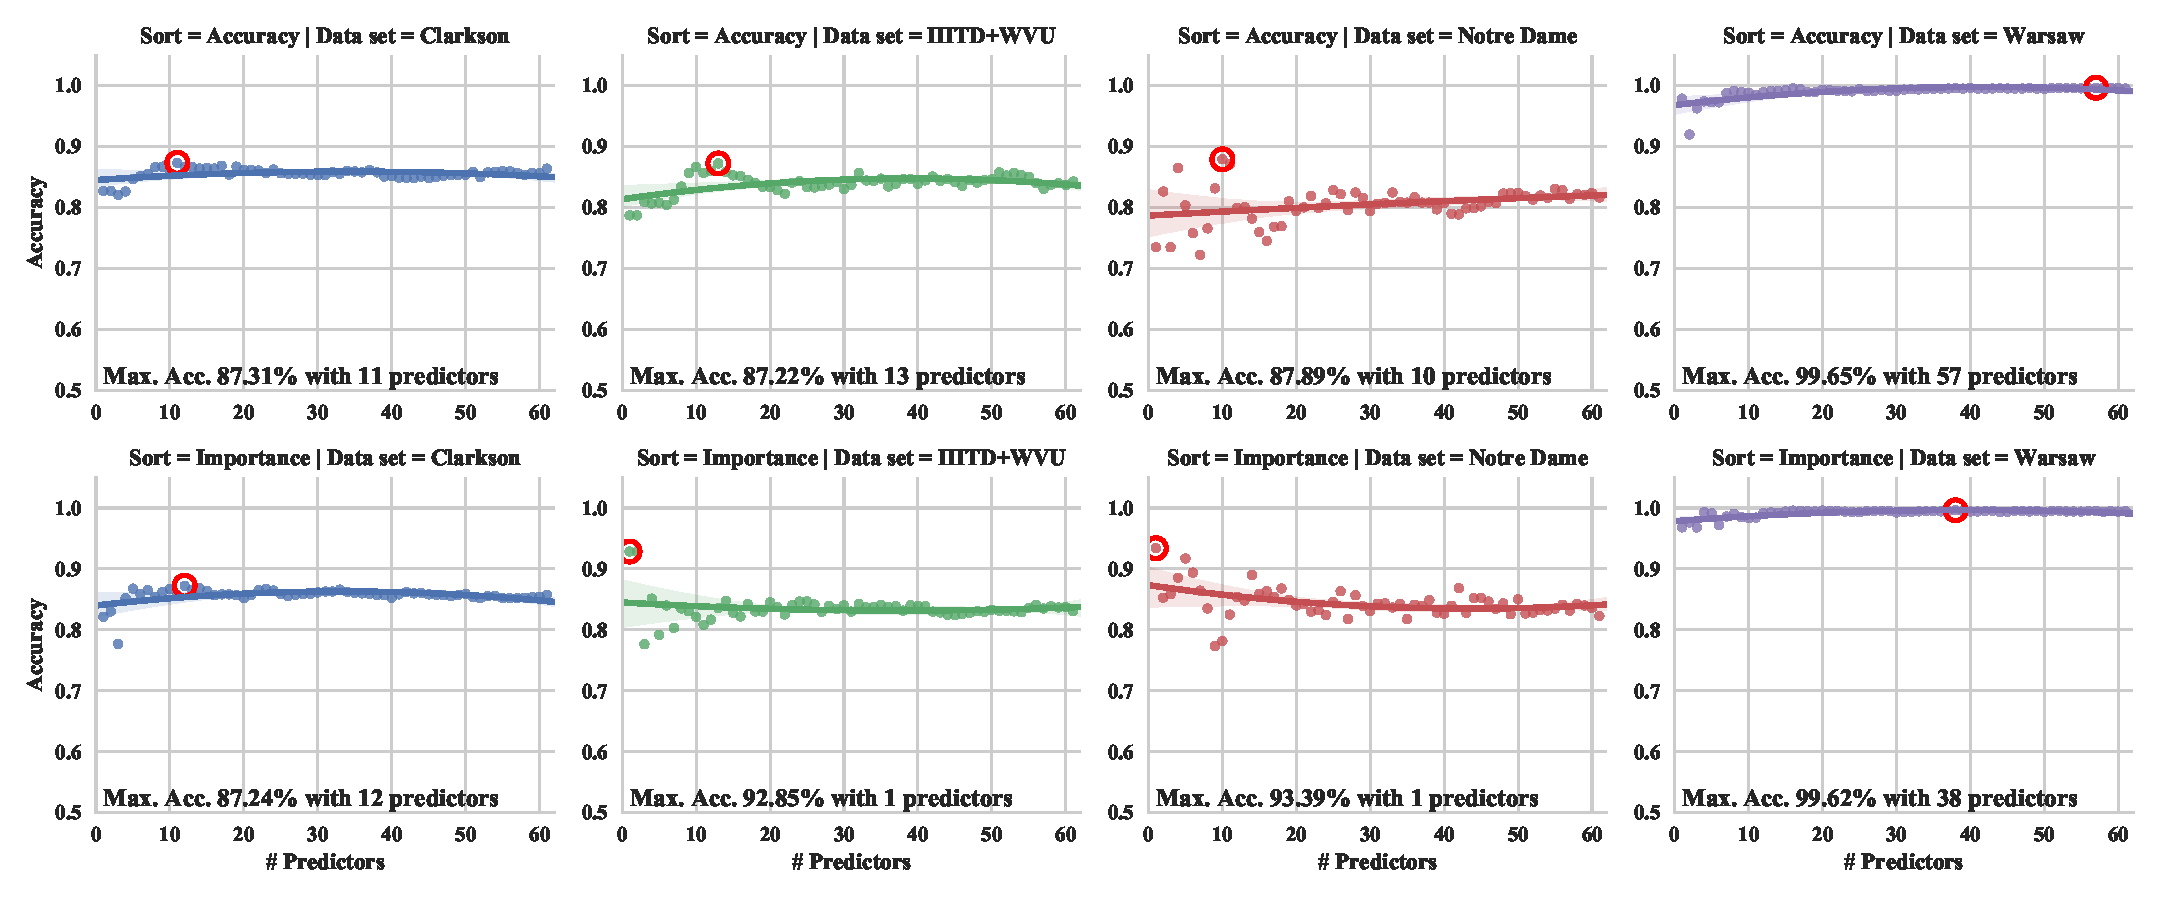
\includegraphics[
        width=\textwidth,
        trim=0.5cm 0cm 0.5cm 1cm
    ]{incremental_weighted_voting_fusion}
    \caption{Relationship between classification accuracy and number of predictors used in the fusion. The top row shows results for \textit{BWWVA}, and the bottom row for \textit{BWWVI}.}
    \label{fig:incremental_fusion}
\end{figure*}

These somehow contradictory results motivated us to further investigate this aspect.  Fig.~\ref{fig:incremental_fusion} shows the relationship between the number of predictors and the output accuracy, for each weighted voting fusion technique and for each data set. 
% The data points show that in almost every case, the combination of a certain number of predictors can be beneficial, but the use of all of them does not always improve accuracy. 
For each fusion method and dataset, after the optimal number of predictors is reached, the addition of extra predictors does not improve the results, and in some cases it may even be detrimental.
In some cases, the optimal accuracy is reached using a single predictor, but other cases may require up to 57 predictors. 

A method for predictor selection is necessary so that we can obtain the best accuracy from the ensemble.
% maximum result from the fusion process. 
However, this process is not trivial: the analysis of the predictor-accuracy relation in other data partitions (train and validation) reveals significantly different trends. Consequently, it is not always possible to determine the optimal number of predictors to be used in the unknown partition by simply using information from other partitions.

Accuracy is the obvious metric of choice for selecting the best base classifiers, but it does not tell us about the complementarity relations between different classifiers. The \textit{Gini} importance measure calculated by training a Random Forest can suggest the best classifiers, based on how much each predictor helps to reduce the impurity in a decision tree. Therefore, it can also be used as a criterion for predictor selection. However, neither of these estimations helps us to determine an optimal number of predictors. Furthermore, our results show there is no distinct advantage in using either accuracy or importance. These results motivated us to search for a method for selection of predictors that is based on their already known properties, but also based on how different base classifiers integrate with each other. 


% ==========================================================================================================
\subsection{Cross-Domain Evaluation}
\label{sec:cross_dataset_evaluation}

With the exception of Clarkson, all LivDet-Iris 2017 datasets were designed to allow cross-sensor evaluation. Images in their unknown partitions were captured with different sensors and environments. Additionally, we conducted cross-dataset experiments to verify the possibility of transfer learning across these datasets. However, direct cross-dataset evaluation using simple fusion did not result in good accuracy. In fact, training CNN predictors in one data set and testing them in another resulted in accuracy no better than random prediction.

One of the premises of our approach is the use of multiple views of the data, in order to capture texture subtleties. We can confirm this if we consider the ranges of BSIF filter sizes that had better accuracy in the different data sets. This suggests there is enough difference in texture scale from one data set to another to cause the individual CNN predictors not to be able to recognize them. The variation of these data sets in nature (texture contacts, printouts, or a mix of both), composition (regarding sizes of partitions and classes), acquisition devices and environments can explain the limited ability for transfer learning here.

Despite the fact that direct cross-dataset evaluation was not successful, training CNN predictors in a combined dataset produced much better results. Table \ref{tab:combined_results} shows a comparison of all predictors and their fusion in the combined dataset. Both individual CNNs and simple fusion methods achieved typically over $95\%$ classification accuracy in the known test partition. In the unknown partition, while most CNN predictors achieved HTER of $12\%$ or lower, all simple fusion methods obtained HTER below $8\%$, with classification accuracies higher than $91\%$ even on the unknown set. 

\begin{table}[!ht]
\centering
\caption{HTER (\%) on the Combined dataset.}
\label{tab:combined_results}
\begin{tabular}{c|ccccc}
\hline
  &No Fusion & RF    & MV    & BWWVI & BWWVA \\
  &(avg.) \\ \hline
K & 2.57  & 0.74  & 0.65  & 0.59  & 0.63 \\
U & 12.47 & 7.02  & 6.89  & 7.12  & 6.88 \\ \hline
\end{tabular}
\end{table}

% \begin{figure}[ht]
%     \centering
%     \includegraphics[
%         width=\linewidth,
%         trim=0.5cm 0.5cm 0.5cm 0.5cm
%     ]{combined_hter}
%     \caption{HTER on the Combined dataset.}
%     \label{fig:combined_results}
% \end{figure}


\begin{figure*}[ht]
    \centering
    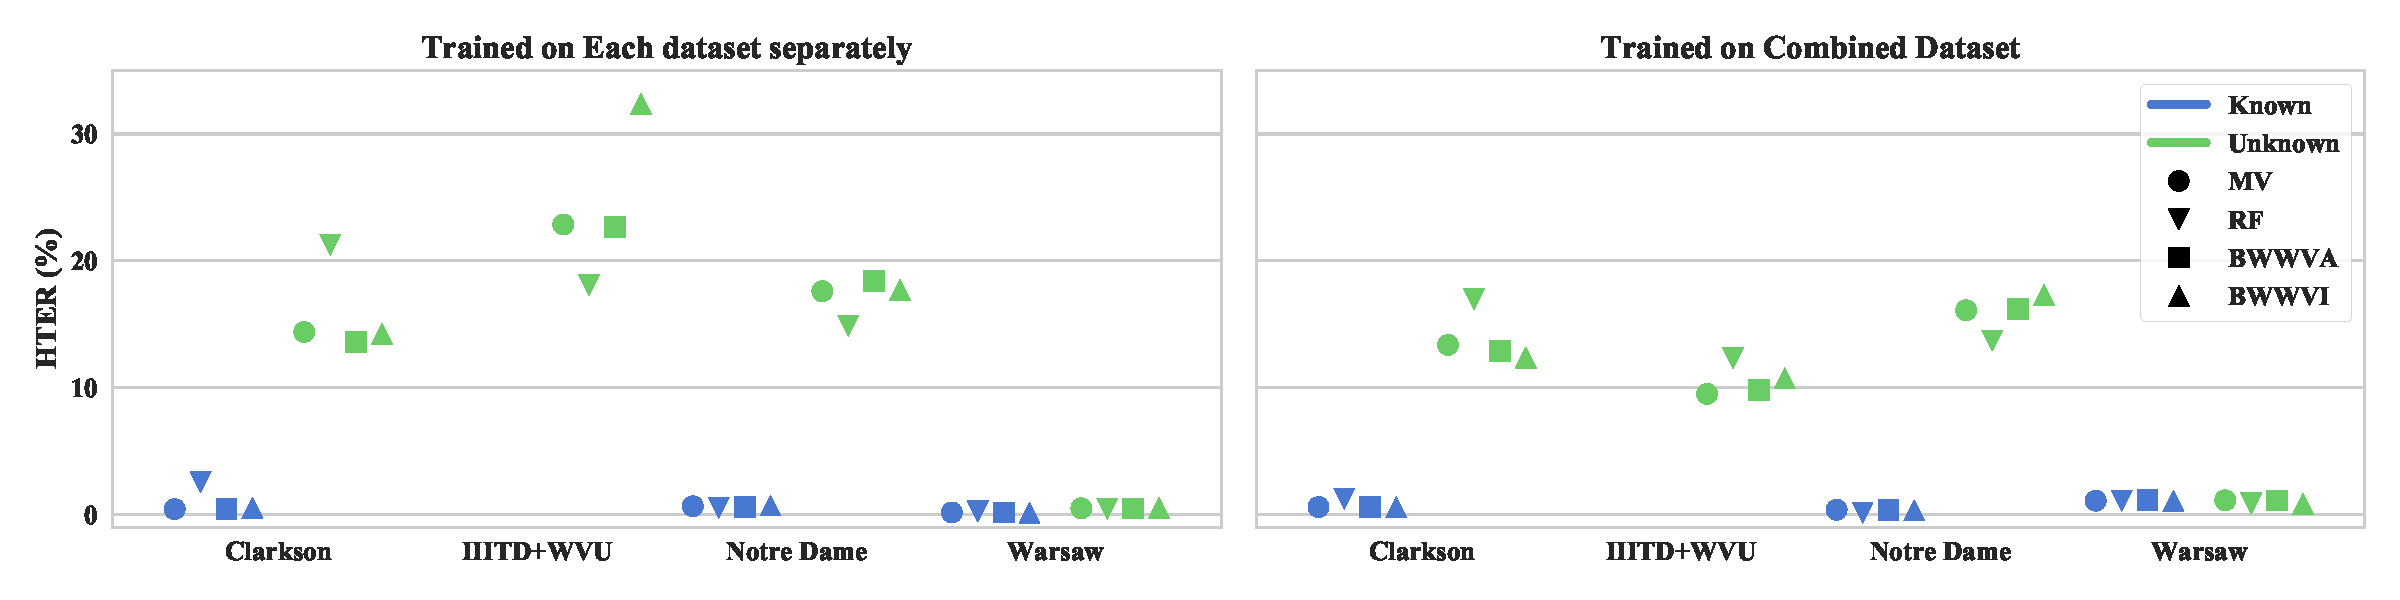
\includegraphics[
        width=\linewidth,
        trim=0.5cm 1cm 0.5cm 0.5cm
    ]{fusion_distrib_train}
    \caption{HTER distribution for fusion methods. On the left, training and evaluation is performed on each individual dataset. On the right, training is performed on the combined dataset, and evaluation is performed on each individual dataset.}
    \label{fig:fusion_distrib}
\end{figure*}


Fig.~\ref{fig:fusion_distrib} shows the distribution of HTER for fusion methods, in a comparison between training on each individual dataset, and training on the combined dataset. Performing the training on the combined dataset was particularly favorable in IIITD+VWU dataset, in which HTER was reduced from more than $25\%$ to nearly $10\%$. 
% \todo[inline]{Perhaps we should eliminate Figs \ref{fig:combined_results} and/or \ref{fig:fusion_distrib}. This section is too crammed. Besides, results in there are almost better than Table III, and we don't want to spoil that. Opinions?\\
% AP: I guess we should move this discussion to the next section and add in this comparison the results obtained using the meta-fusion, which is our best results, actually. Another possibility is to create a new subsection for this discussion, of course, if we have enough material for that.
% }

% ==========================================================================================================
\subsection{Evaluation of the Proposed Meta-Analysis: Selection and Meta-Fusion of Classifiers}
\label{sec:evaluation_meta_analysis}

%
\begin{table*}[!hb]
\centering
\caption{Performance results (\%) of the proposed method, majority vote, and the best individual CNN model for the \emph{test known} (K), \emph{test unknown} (U), and \emph{overall test} (O) partitions from datasets used in this work. The classifiers were trained on the train partition of each dataset. $^\dagger$~IIITD-WVU dataset contains only the \emph{unknown test} partition.}
\setlength{\tabcolsep}{3.5pt}
\begin{tabular}{cc||c|c|c||c|c|c||c|c|c||c|c|c}
    \toprule
				     & 						& \multicolumn{3}{c||}{\textbf{Meta-Fusion via SVM}} 
										    & \multicolumn{3}{c||}{\textbf{BWWVA}}
										    & \multicolumn{3}{c||}{\textbf{RF}}
										    & \multicolumn{3}{c}{\textbf{Best Individual CNN}} \\

    \textbf{Dataset} & \textbf{Testing set} & \textbf{APCER} & \textbf{BPCER} & \textbf{HTER} 
                                            & \textbf{APCER} & \textbf{BPCER} & \textbf{HTER} 
                                            & \textbf{APCER} & \textbf{BPCER} & \textbf{HTER} 
                                            & \textbf{APCER} & \textbf{BPCER} & \textbf{HTER} \\
    \hline\hline
			                    & K    & 0.00    & 2.44    & 1.22    & 0.33    & 0.89    & 0.61	   & 0.44   & 0.67  & 0.56  & 0.67    & 2.44    & 1.56    \\
    Notre Dame            		& U    & 9.22    & 1.44    & 5.33    & 35.78   & 1.00    & 18.39   & 29.33  & 0.44  & 14.89 & 32.44   & 2.44    & 17.44   \\
							    & O    & 4.61    & 1.94    & 3.28    & 18.06   & 0.94    & 9.50	   & 14.89  & 0.56  & 7.72  & 16.56   & 2.44    & 9.50    \\
    \midrule                               	
								& K    & 0.05    & 0.82    & 0.44    & 0.05    & 0.31	 & 0.18	   & 0.05   & 0.51  & 0.28  & 0.30    & 0.41    & 0.35    \\
    Warsaw                		& U    & 0.09    & 1.49    & 0.79    & 0.37	   & 0.60	 & 0.48    & 0.32   & 0.64  & 0.48  & 20.97   & 0.68    & 10.83   \\
						        & O    & 0.07    & 1.29    & 0.68    & 0.21	   & 0.45	 & 0.33	   & 0.19   & 0.58  & 0.38  & 10.63   & 0.55    & 5.59    \\
    \midrule                    
                                & K    & 4.55    & 0.20    & 2.37    & 0.00    & 0.94    & 0.47	   & 3.48   & 0.47  & 1.98  & 1.26    & 1.75    & 1.50    \\
    Clarkson              		& U    & 41.54   & 0.31    & 20.92   & 26.30   & 0.63    & 13.47   & 39.12  & 0.63  & 19.88 & 32.71   & 1.88    & 17.29   \\
								& O    & 18.66   & 0.24    & 9.45	 & 13.30   & 0.78    & 7.04	   & 21.30  & 0.55  & 10.93 & 16.98   & 1.82    & 9.40    \\
    \midrule
								& U    &  	     &         &         &         &         &         &        &       &       &         &         &         \\
    \multirow{-2}{*}{IIITD+WVU~$^\dagger$} 
                                & O    & \multirow{-2}{*}{12.32}	
												 & \multirow{-2}{*}{17.52}
												 & \multirow{-2}{*}{14.92}
												 & \multirow{-2}{*}{12.29}
												 & \multirow{-2}{*}{33.05}
												 & \multirow{-2}{*}{22.67}
												 & \multirow{-2}{*}{5.56}
												 & \multirow{-2}{*}{21.23}
												 & \multirow{-2}{*}{13.39}
												 & \multirow{-2}{*}{21.81}
												 & \multirow{-2}{*}{72.22}
												 & \multirow{-2}{*}{47.02} \\
    \hline
    \hline
    Average						& O    &\bf 8.92 &\bf 5.25 &\bf 7.08 & 10.96   & 8.80   & 9.88   & 10.48    & 5.73  & 8.11  & 16.50	& 19.26	  & 17.88     \\
    \bottomrule
\end{tabular}\\
\label{tab:meta_classification_results}
\end{table*}


In this section, we evaluate the proposed method designed to automatically select the most relevant multi-view-CNN predictors, in terms of their importance and complementarity, and to fuse their individual results via meta-fusion approach, which was performed using the Support Vector Machine.

First, we used our proposed algorithm described in Section~\ref{subsec:meta_fusion_algorithm} to select the most relevant predictors from a pool of $61$ predictors. Next, we performed a meta-fusion using the SVM with a radial basis function kernel. Both the parameters of the SVM and the parameter \textit{k} (see Sec.~\ref{subsec:meta_fusion_algorithm}) were found through grid search in the aggregated training sets of all datasets considered in this work. The \emph{known} and \emph{unknown} test sets were used only to report the final performance results.

\mathchardef\mhyphen="2D  % https://www.logic.at/staff/salzer/etc/mhyphen/
% Fig.~\ref{fig:meta_fusion_grid_search} shows results, in terms of HTER, of different values for \textit{k} considering the training data. 
We performed a fine grid-search of parameter \textit{k} on the neighborhood of (5, 20), and the best HTER was achieved with $k=16$.
According to one-sample Wilcoxon signed-rank test, the observed differences in the HTER values obtained for each $k$ are statistically significant at the significance level $\alpha=0.05$ ($p\mhyphen value=0.0004$). Henceforth, we use $k=16$ to report performance results of our proposed method.

Furthermore, Table~\ref{tab:meta_classification_results} shows the effectiveness of our meta-fusion approach compared to the best multi-view-CNN predictor and the majority vote fusion technique. In addition to the results for \emph{test known} and \emph{test unknown} partitions, Table \ref{tab:meta_classification_results} also presents \emph{overall test}, which corresponds to the accuracy obtained on both test partitions combined. These results are in agreement with those reported in the literature~\cite{kuncheva2014}, which states that both accuracy and complementarity are the foundation for effective fusion.

% ==========================================================================================================
\subsection{Comparison with the State of the Art}
\label{sec:comparison_sota}

In this section, we compare our results with the LivDet-Iris 2017 best performing method. As we can see, our method outperforms the competition winner. Table \ref{tab:livdet} summarizes the results of the competition in contrast to our best solution developed solely on the LivDet-Iris 2017 train partitions.

Even in the cases where our methods were not able to outperform one of the specific error rates, we were able to significantly reduce the combined error rate. This happens, for instance, in the overall performance on IIITD+WVU dataset: the best HTER among LivDet-Iris 2017 competitors is $16.7\%$. Although our methods did not outperform their BPCER of $3.99\%$, we managed to lower HTER to $7.9\%$ on that specific dataset. Similar situations occurred on all datasets, showing a consistent improvement of our results over the state of the art.

\newcommand{\specialcell}[2][c]{%
  \begin{tabular}[#1]{@{}c@{}}#2\end{tabular}
}

\begin{table}[!htb]
	\centering
	\caption{Comparison of HTER (\%) with LivDet-Iris 2017, on the combined \emph{test known} and \emph{test unknown} partitions.}
	\label{tab:livdet}
	\begin{tabular}{cccc}
		\topline
						 &                           & \textbf{Proposed}      & \\
		\textbf{Dataset} & \textbf{LivDet-Iris 2017} & \textbf{Meta-Fusion}   & \textbf{Error} \\
						 & \textbf{Winner}           & \textbf{approach} 	  & \textbf{Reduction (\%)} \\
		\hline\hline
			Clarkson   & 9.59   & 9.45	&  1.46  \\
			\hline
			IIITD+WVU  & 16.70  & 14.92	&  10.66 \\
			\hline
			Notre Dame & 4.03   & 3.28	&  18.61  \\
			\hline
			Warsaw     & 5.81   & 0.68	&  88.30  \\
			\hline\hline
			Average    & 9.03   & 7.08	&  21.59   \\
			\bottomrule
	\end{tabular}
\end{table}

Meta-Fusion results were further improved when applied to the combined dataset. Table \ref{tab:combined-meta} presents these results in comparison with LivDet-Iris 2017, and also with our previous Meta-Fusion results. The overall HTER was reduced from $7\%$ to $4\%$ when Meta-Fusion was applied to the combined dataset. At this point, it is necessary to be clear about the LivDet-Iris 2017 comparison: the known and unknown HTER numbers presented in Table \ref{tab:combined-meta} are estimated. Since BPCER is not available for all \emph{known} and \emph{unknown} test partitions in LivDet-Iris 2017, we assumed 0 (perfect score) in our estimation. Even with this optimistic assumption about the competition results, our method achieved an error reduction of more than $50\%$ with regard to the former.

Our current implementation takes, on average, 0.028s to perform classification on a single image. Timing was performed on a 4-core Intel(R) Xeon(R) CPU E5-2650 v4 @ 2.20GHz with 128GB of RAM, equipped with a GeForce GTX 1080 Ti GPU. This time includes the CNN classification of the 61 data views and the meta-fusion of their results. Since the LivDet-Iris protocol does not establish parameters for speed efficiency analysis, the main directive for our implementation herein was classification accuracy. Therefore our method's efficiency can certainly be optimized, if needed. 

\begin{table}[ht]
    \begin{minipage}{\linewidth}
	\centering
	\caption{Results in terms of HTER (\%) for our Meta-Fusion approach trained on the Combined dataset. Error reduction (ER) values present the error decrease achieved by our approach with regard to LivDet-Iris 2017 winner.}
	\label{tab:combined-meta}
    \begin{tabular}{cccccc}
        \topline
                         &                           & \multicolumn{4}{c}{\textbf{Proposed Meta-Fusion approach (\%)}} \\
                         
        \cline{3-6}
                         & \textbf{LivDet-Iris 2017} & \multicolumn{2}{c}{\textbf{Trained on}} & \multicolumn{2}{c}{\textbf{Trained on}} \\
        \textbf{Dataset} & \textbf{Winner}           & \multicolumn{2}{c}{\textbf{each dataset}} & \multicolumn{2}{c}{\textbf{Combined dataset}} \\
						 & \textbf{HTER}             & \textbf{HTER} 	  & \textbf{ER}  & \textbf{HTER} 	  & \textbf{ER} \\
        \hline\hline
        K   & 0.74\footnote{Estimated\label{fn:1}}  & 1.34          & -81.08        & 0.74 & 0.00 \\
        U   & 13.23\textsuperscript{\ref{fn:1}}     & 10.49         & 20.71         & 8.39 & 36.58 \\
        O   & 9.03                                  & 7.08          & 21.59         & 4.44 & 50.83 \\
        \bottomrule
    \end{tabular}
    \end{minipage}
\end{table}
